% 
% Annual Cognitive Science Conference
% Sample LaTeX Paper -- Proceedings Format
% 

% Original : Ashwin Ram (ashwin@cc.gatech.edu)       04/01/1994
% Modified : Johanna Moore (jmoore@cs.pitt.edu)      03/17/1995
% Modified : David Noelle (noelle@ucsd.edu)          03/15/1996
% Modified : Pat Langley (langley@cs.stanford.edu)   01/26/1997
% Latex2e corrections by Ramin Charles Nakisa        01/28/1997 
% Modified : Tina Eliassi-Rad (eliassi@cs.wisc.edu)  01/31/1998
% Modified : Trisha Yannuzzi (trisha@ircs.upenn.edu) 12/28/1999 (in process)
% Modified : Mary Ellen Foster (M.E.Foster@ed.ac.uk) 12/11/2000
% Modified : Ken Forbus                              01/23/2004
% Modified : Eli M. Silk (esilk@pitt.edu)            05/24/2005
% Modified: Niels Taatgen (taatgen@cmu.edu) 10/24/2006

%% Change ``a4paper'' in the following line to ``letterpaper'' if you are
%% producing a letter-format document.

\documentclass[10pt,letterpaper]{article}

\usepackage{amsmath, amssymb}
\usepackage{cogsci}
\usepackage{pslatex}
\usepackage{apacite}
\usepackage{graphicx} 
\usepackage{natbib}
\usepackage{pseudocode}
\usepackage[font=small,skip=5pt]{caption}

\renewcommand{\topfraction}{0.9}	% max fraction of floats at top
\renewcommand{\bottomfraction}{0.8}	% max fraction of floats at bottom
%   Parameters for TEXT pages (not float pages):
\setcounter{topnumber}{2}
\setcounter{bottomnumber}{2}
\setcounter{totalnumber}{4}     % 2 may work better
\setcounter{dbltopnumber}{2}    % for 2-column pages
\renewcommand{\dbltopfraction}{0.9}	% fit big float above 2-col. text
\renewcommand{\textfraction}{0.07}	% allow minimal text w. figs
%   Parameters for FLOAT pages (not text pages):
\renewcommand{\floatpagefraction}{0.7}	% require fuller float pages
% N.B.: floatpagefraction MUST be less than topfraction !!
\renewcommand{\dblfloatpagefraction}{0.7}	% require fuller float pages
\setlength{\parskip}{2mm plus1mm minus0mm}
%\setlength{\textfloatsep}{\baselineskip plus 0.2\baselineskip minus 0.2\baselineskip}


\newcommand{\eg}{e.g. }
\newcommand{\ie}{i.e. }
\newcommand{\fg}{Fig.}
\newcommand{\corevectors}{core}
%\newcommand{\inverseop}[1]{\mathbf{#1}'}
\newcommand{\inverseop}[1]{\overline{\mathbf{#1}}}
\newcommand{\synset}[1]{\textbf{#1}}
\newcommand{\relation}[1]{\textbf{#1}}
\newcommand{\unbinding}{unbinding}
\newcommand{\rel}{rel}
\newcommand{\sub}{subj}
\newcommand{\obj}{obj}
\newcommand{\Sarah}{Eve}
\newcommand{\Fido}{Max}


\title{Learning Structured Information in Spiking Neurons}
 
%\setlength{\textfloatsep}{5pt plus 1.0pt minus 2.0pt}
\author{\large \bf Eric Crawford (e2crawfo@uwaterloo.ca)\\
  \large \bf Chris Eliasmith (celiasmith@uwaterloo.ca)\\
  Centre for Theoretical Neuroscience, University of Waterloo,
  Waterloo, ON, N2L 3G1}
\setlength{\intextsep}{1pt plus 1.0pt minus 2.0pt}
\setlength{\textfloatsep}{5pt plus 1.0pt minus 2.0pt}
%\setlength{\textfloatsep}{.1cm}
\begin{document}


%\abovedisplayskip=1pt

\maketitle

\begin{abstract}
Because it provides no straightforward characterization of symbolic processing, connectionism generally struggles to provide a convincing account of the human ability to learn, represent and manipulate structured information. Moreover, while some models have been successful at giving an account of how neurons can \textit{represent} structured knowledge, such approaches generally fail to give a convincing account of how this representation can be learned from experience in the environment. Here, we provide such an account. In a previous paper, we showed how to use a combination of Vector Symbolic Architecture and a sophisticated technique for neural representation to construct a spiking neural network capable of efficiently representing a human-scale semantic network \citep{crawford2013}. In the present work, we expand on this approach, showing how this neural network can be learned from input data, using biologically plausible neural learning rules. We demonstrate the success of our technique by having it learn to encode randomly generated structured knowledge bases, and provide arguments suggesting that this approach will scale up to learning knowledge bases as big as a human vocabulary.

\textbf{Keywords:} 
knowledge representation; biologically plausible; scaling; neural; vector symbolic; plasticity; learning
\end{abstract}

\section{Introduction}
Learning large-scale structured information is one of the most impressive human abilities. It is also one of the abilities that is hardest to account for in terms of neural computation, largely owing to the fact that connectionism provides no straightforward account of structural learning or representation. In a previous paper, we demonstrated one approach to \textit{representing} large structured knowledge bases \citep{crawford2013}. Our technique was an improvement on all past efforts in this domain, in terms of both ability to scale and biological plausibility. The technique we presented there relied in large part on a large associative memory, and the efficient scaling was largely due to a novel technique for storing associations in spiking neurons. However, one shortcoming of the technique was that the connection weights in the network were computed offline using neural engineering techniques, and it was left as an open question whether such a representation could be learned in a biologically plausible manner from experience. Here we directly address this issue, showing that the association module of this network can indeed be learned in a biologically plausible manner.

We begin by presenting the outline of our technique for representing structured knowledge neurally, demonstrating why  an efficient neural associative memory is vital for the success of the network. We then present a technique showing how such a memory can be learned in a neuron-efficient manner. We conclude by showing the results of simulations conducted using this technique, to solve a task that emulates a child learning semantic structure.

\section{Vector Encoding of Structured Knowledge}
We begin by presenting a formalism that allows the encoding of large structured knowledge bases, such as a semantic network, in a vectorial format. When combined with the Neural Engineering Framework \citep{Eliasmith2003m}, a principled way of representing vectors in spiking neurons, this formalism will act as a bridge between the previously disparate realms of spiking neural computation and large, structured knowledge bases.

\subsection{Holographic Reduced Representations}
Holographic Reduced Representations (HRRs) are a type of Vector Symbolic Architecture (VSA). They provide us with a means of representing structured knowledge in a vectorial format \citep{Plate2003d}.  To begin, we fix a dimension for our vectors. 
Previous investigations have shown that using 512-dimensional vectors provides sufficient representational capacity to accommodate knowledge bases containing on the order of 60,000 items \citep{Eliasmith2012}, roughly the size of an adult human vocabulary \citep{Ogrady}. However, computational constraints have not permitted us to use such large knowledge bases in the present study (though we do give reasons why our approach should gracefully scale up to knowledge bases this large), rendering 512-dimensions excessive. Consequently, here we use 64-dimensional vectors. 

Each symbol in the structured knowledge base that we want to represent is then assigned two vectors. The first is called an ID-vector, and acts as a unique identifier for the symbol it is assigned to. The second vector is an HRR that encodes the structured relations belonging to the symbol it is assigned to. This vector is built up in terms of ID-vectors corresponding to related symbols and other vectors assigned to relations, combined using specialized operations specified by the HRR formalism.

Suppose, for example, that our vocabulary contains a symbol \textit{dog}, and we would like to encode two facts or relations about dogs, namely that they are members of packs, and that they are canines. Using the HRR operations of \textit{circular convolution} ($\circledast$) and \textit{vector addition} ($+$), the HRR for \textit{dog} is given by:
\begin{align}
  \mathbf{dog} = \mathbf{isA} \circledast \mathbf{canine_{ID}} + \mathbf{partOf} \circledast \mathbf{pack_{ID}}\label{eqn:dog-sem}
\end{align}
For the rest of the paper, all vectors appear in bold, and ID-vectors are denoted with the \textbf{ID} subscript to distinguish them from HRR vectors. 

In general, for each relation belonging to a symbol we want to represent, the HRR for that symbol contains a term consisting of a relation vector circularly convolved with the ID-vector for the target of the relation. An important note is that \textbf{dog} in Equation \eqref{eqn:dog-sem} has the same dimensionality as each of the vectors on the right-hand side of the equation. This feature has a number of desirable consequences which set HRR's apart from other VSA's. For instance, any structures we build to manipulate HRR's can assume vectors of a fixed dimensionality. More importantly, this prevents the size of the vectors from undergoing a combinatorial explosion as the depth of the knowledge structure increases, permitting the representation of deeply hierarchical structures.

What makes HRR's useful is that the \textbf{dog} vector preserves information about its constituents; given a relation vector (e.g., \textbf{isA}, \textbf{partOf}), we can use a third operation, \textit{deconvolution} to extract the vector that that relation vector is convolved with in \textbf{dog}; in short, it allows the extraction of the relational information stored in \textbf{dog}. Deconvolution amounts to performing circular convolution between the HRR and the inverse of the relation vector, denoted by an overbar. For example, if we want to extract the symbol that \textbf{dog} is related to via the \textbf{isA} relation, we circularly convolve \textbf{dog} with $\overline{\mathbf{isA}}$:
\begin{align}
&\mathbf{dog} \circledast \overline{\mathbf{isA} }\notag\\
&=(\mathbf{isA} \circledast \mathbf{canine_{ID}} + \mathbf{partOf} \circledast \mathbf{pack_{ID}}) \circledast \overline{\mathbf{isA} }\notag\\
&=\mathbf{isA} \circledast \mathbf{canine_{ID}} \circledast \overline{\mathbf{isA} } + \mathbf{partOf} \circledast \mathbf{pack_{ID}} \circledast \overline{\mathbf{isA} }\notag\\
&\approx \mathbf{canine_{ID}} + \mathbf{partOf} \circledast \mathbf{pack_{ID}} \circledast \overline{\mathbf{isA} }\label{eqn:unbind}
\end{align}
yielding a vector that is similar to $\mathbf{canine_{ID}}$. However, there is still some work to do to fully extract the relational information from \textbf{dog}, partly due to the other terms present.

\subsection{Associative Memories}
The result of deconvolution (equation \eqref{eqn:unbind}) is insufficient in two ways. First, because of the other terms, it is only \textit{similar to} $\mathbf{canine_{ID}}$; in other words, there is noise the must be removed. Second, $\mathbf{canine_{ID}}$ is not particularly useful on its own; it would be much more useful to have the HRR for canine, from which we could recursively extract further structural information. These problems can be solved simultaneously by an associative memory.

Associative memories typically store ordered pairs of vectors $\langle\xi, \eta\rangle$. When the memory receives an input, if that input is sufficiently similar to some $\xi$, then the memory outputs the corresponding $\eta$. It is easy to see how this solves our problems if we let the $\xi$ be ID-vectors and the $\eta$ be HRR's: the associativity provides the mapping, and the fact that the input only has to be suffuciently similar to some $\xi$ solves the denoising problem. 

For example, for our miniature dog-centric vocabulary, the pairs stored in the associative memory would be $\langle\mathbf{dog_{ID}}, \mathbf{dog}\rangle$, $\langle\mathbf{canine_{ID}}, \mathbf{canine}\rangle$ and $\langle\mathbf{pack_{ID}}, \mathbf{pack}\rangle$. When the vector from Equation \eqref{eqn:unbind} is given as input, it will be similar to $\mathbf{canine_{ID}}$, and disimilar to $\mathbf{dog_{ID}}$ and $\mathbf{pack_{ID}}$. Consequently, the output of the associative memory will be $\mathbf{canine}$.

A significant portion of this paper is concerned with demonstrating how a scalable, efficient, biologically-plausible neural associative memory can be learned from training data.

\section{Learning Structured Knowledge in Spiking Neurons}
We begin this section with a characterization of a framework that provides a principled approach to constructing networks of spiking neurons that represent and transform high-dimensional vectors, including those used in the vectorial encoding of structured knowledge given in the previous section. We then show how to apply this approach to build a spiking neural network capable of learning arbitrary associations.

\subsection{Neural Representation and Computation}
The Neural Engineering Framework (NEF) is a set of methods for building biologically
plausible models using principles for neural representation, transformation and dynamics \citep{Eliasmith2003m}. 
The central idea behind the NEF is that the activity of a population of spiking neurons can be interpreted as representing a vector whose dimensionality is potentially much different from the size of the neural population; a typical case is to have a 2-D vector represented by a population of 100 spiking neurons. The NEF then provides a set of methods for determining connection weights between neural populations which compute any desired function of the represented vector.

Suppose, for instance, that we have a population A representing some vector $x$, and that we would like a second population B to represent $f(x)$, an arbitrary function of $x$. The NEF tells us exactly what the feedforward connection weights between A and B must be to compute this function. To achieve this, the NEF assumes that each neuron in A and B has an \textit{encoding} vector, sometimes called a \textit{preferred direction vector}, which specifies the direction in the represented space of the population for which the neuron is most active. The spiking activity of every neuron in a population A can be written:
\begin{align}
a_i (x) = G [\ \alpha_i e_i x\ +\ J_{bias}\ ]\label{eqn:enc}
\end{align}
where $a_i$ is the spiking activity of $i$th neuron in the population, $G$ is the spiking neural nonlinearity, $\alpha_i$ is the gain of the neuron, $e_i$ is the encoding vector of the $i$th neuron, and $J_{bias}$ is a bias current to account for background activity of the neuron. The elements in the square brackets correspond to the current flowing into the cell, which then drives the spiking of the chosen single cell model $G$. For computational efficiency, we employ a leaky integrate-and-fire (LIF) neuron model, though the NEF can be applied for arbitrary neuron models. Equation \eqref{eqn:enc} is referred to as the \textit{encoding} equation because it describes how a vector, in this case $x$, is encoded into neural spikes. The NEF then assumes linear decoding can be used to reconstruct $x$ or any nonlinear function thereof, $f(x)$, from the spiking activity of the population. Thus, we assign each neuron a
\textit{decoding} vector $d^f_i$, which are used to obtain a reconstruction of $f(x)$, denoted here as $\widehat{f(x)}$, in terms of the activities of the population:
\begin{align}
\widehat{f(x)} = \sum_i a_i(x) d^f_i \label{eqn:dec}
\end{align}
where $N$ is the number of neurons in the population. This is known as the \textit{decoding} equation, since it describes how the activity of a population can be decoded to obtain an estimate of the value of a function of the vector currently represented by the population. The NEF assumes that the decoders are obtained through a least-squares optimization process, performed offline before the network is created. This is done by minimizing the equation:
\begin{align}
E = \frac{1}{2}\int[f(x) - \sum_i a_i(x) d^f_i]^2dx\label{eqn:error}
\end{align}
with respect to $d^f_i$.
Recall that our purpose is toderive connection weights between A and B that compute the function $f$ on the vector represented by A. If we define the encoding
and decoding for populations A and B using equations \eqref{eqn:enc} and \eqref{eqn:dec}, we can substitute the
decoding of A into the encoding of B, thereby deriving connection weights. The weights for computing $f$ are then:
\begin{align}
\omega_{ij} = \alpha_j e_j d^f_i \label{eqn:weight}
\end{align}
where $i$ indexes the neurons in A and $j$ indexes the neurons in B. Intuitively, this weight matrix works by decoding $f(x)$ from population A using the decoding vectors for the neurons in A, and encoding it into the activities of population B using the encoding vectors for the neurons in B.

\subsection{Learning Associations in Spiking Neurons}
We now show how this technique, combined with neural learning rules, can be applied to create a spiking neural network capable of efficiently learning associations. Given $N$ pairs of vectors to associate, $\langle\xi_k, \eta_k\rangle$ for $k \in 1 \dots N$, the following simple algorithm implements the associative memory functionality:
 
\renewcommand{\thepseudocode}{1}

\begin{pseudocode}[ruled]{Association}{v}
  \label{alg:simple}
  sum \GETS 0\\
  \FOR k \GETS 1 \TO N\\
  \BEGIN
    scale \GETS threshold(\xi_k \cdot v) \\
    sum \GETS sum + scale * \eta_k\\
  \END\\
  \RETURN{sum}
\end{pseudocode} 

If the threshold is set correctly (which depends on the statistics of the input), \textit{scale} will be non-zero for at most one value of $k$, and the output will be either the zero vector or $\eta_k$.

In previous work, the NEF has been used to construct a network implementing a neural variant of this algorithm, and the resulting network has been shown to posses a number of unique advantages. \citet{crawford2013} demonstrated its scalability, using the technique to create a network accurately encoding WordNet, a semantic network containing $\sim$117,000 terms, using only 20 neurons per term. \citet{Stewart2010} demonstrated that this approach significantly outperforms a linear associator, a direct function approximator and a standard multi-layer perceptron in terms of accuracy. It also has an advantage in terms of biological plausibility, since it is implemented in spiking neurons.

In the NEF-constructed neural network implementing this algorithm, each pair of vectors $\langle\xi, \eta\rangle$ is assigned a small ($\sim$20) neural population. The encoding vectors of this population are set equal to $\xi$, and the parameters of the neurons' LIF response functions are set so that the neurons only spike if the input is sufficiently similar to $\xi$. Finally, the decoders of the population are set equal to $\eta$. The overall effect is that when a population is active, it outputs its assigned $\eta$, and a population is active if and only if the input is sufficiently similar to its assigned $\xi$. All these populations converge on a single output population, where the inputs are summed by the dendrites. In essence, each neural population computes, in parallel, one iteration of the loop in Algorithm \ref{alg:simple}.

The associative memory learned by our network employs these same principles. However, rather than computing the appropriate connection weights ahead of time using the NEF as we have done previously, here we want our network to arrive at them through training and the application of learning rules. A schematic diagram of the network that achieves this learning is shown in \fg~\ref{fig:schematic}. 

We impose several assumptions on the pre-trained network. First, we assume that the association population contains a number of neurons that is linear in the number of vectors we want to store. In the future, it is likely that this simplifying assumption can be relaxed, and the appropriate number of neurons allocated online through neurogenesis. Second, we assume that the association population initially employs a sparse representation, such that only a few association neurons are active for any given input vector. Importantly, this initial sparseness is general; roughly the same number of neurons should be active for any input vector, and hence the initial network is equally well equipped to learn any set of associations. The final constraint on the initial network is that the connection weights between the association population and the output population are very small; the effect is that in the early stages of training, no activity in the association population is sufficient to elicit activity in the output population. These initial constraints are enforced by using the NEF to choose encoders and decoders appropriately. We now outline methods by which the initial connection weights in this network of spiking neurons are modified in response to training input to produce a resource-efficient, robust associative memory.

\begin{figure}[b]
\begin{center}
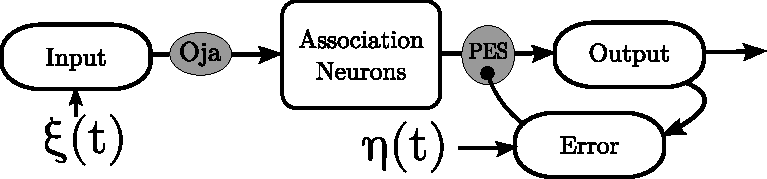
\includegraphics[width=0.5\textwidth]{../diagrams/schematic.pdf}
%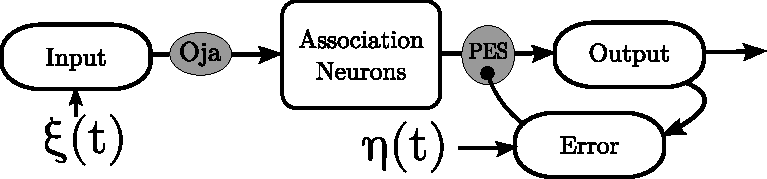
\includegraphics[width=\textwidth]{../diagrams/schematic.pdf}
\end{center}
\caption{Schematic diagram of association network. White rectangles indicate populations of spiking neurons, arrows indicate all-to-all connections between populations, and grey ellipses indicate learning rules applied to connections.}
\label{fig:schematic}
\end{figure}
\subsubsection{Training}
During training, the network has two inputs: $\xi$, the address vector, and $\eta$, the vector to be associated with $\xi$. We present each pair for one second of simulation time, and allow the network to adjust its connection weights.

\subsubsection{Sparse Representation}
The initially sparse representation in the association layer ensures that only a few association neurons are active for any $\xi$ presented during training. These active neurons can be thought of as the neurons assigned to the current pairing. With Algorithm \ref{alg:simple} and its neural equivalent in mind, the goal is now to set the encoders of this population equal to $\xi$, and set the decoders of this population equal to $\eta$, using biologically plausible learning rules. 

\subsubsection{Oja's Rule: Increasing Selectivity}
The first step is to make the active association neurons more selective for the current $\xi$. This may seem redundant, as the sparse representation ensures that the neurons are already fairly selective for the current input vector. However, those active neurons will also respond to other vectors that we might try to store in our memory, which could cause multiple association populations to become active when the memory is used. Our goal here is to ensure that these neurons are active only for input vectors that have a high-degree of similarity to the current training vector. Once training is complete, we want it to be the case that this population is active if and only if the input is a noisy version of the vector the population is assigned to, and thus will have no effect on the output otherwise.

To achieve this increase in selectivity, we use a normalized hebbian learning rule known as Oja's Rule \citep{oja}, applying it to the connections weights between the input and association populations. The ``normalized'' feature of the rule ensures that the connection weights do not grow arbitrarily, which is a major shortcoming of hebbian learning in its simplest form. The weight-update equation employed by Oja's rule is:
\begin{align}
  \Delta w_{ij} = \alpha (x_i y_j - \frac{y_j^2 w_{ij}}{\beta})
\end{align}
where $x_i$ is the activity of the $i$th neuron in the input population, $y_j$ is the activity of the $j$th association neuron, $\alpha$ is the learning rate, and $\beta$ is a constant that is asymptotically proportional to $\sum_i w_{ij}^2$, the sum of squares for each row of the weight matrix. Because the neurons are spiking, the activities $x_i$ and $y_j$ are low-pass filtered versions of spike trains. Fig. \ref{fig:oja} shows an example of what can be achieved by Oja's rule. Because of the form of Oja's rule, only weights for active association neurons are changed; they are increased if the corresponding input neuron is also active, and pushed towards 0 otherwise. During presentation of a noisy version $\xi$, many of the same input neurons will be active, which should active the same set of association neurons.
\begin{figure}[ht]
\begin{center}
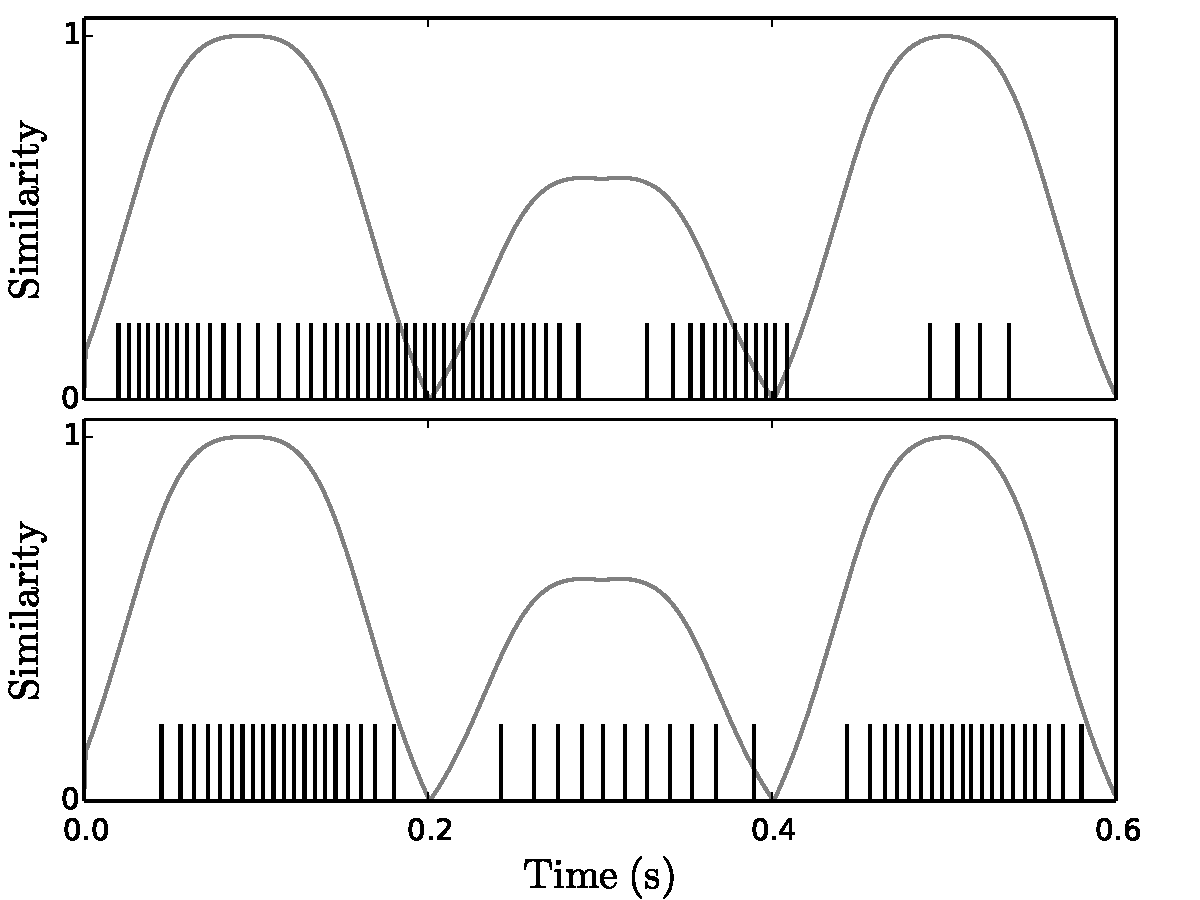
\includegraphics[width=0.5\textwidth]{../default_plots/oja_plot_D_64.pdf}
\end{center}
\caption{Oja's rule changes neural selectivity. A population of neurons capable of representing a 64 dimensional vectors is connected to a single association neuron. Training phase: connection weights between population and association neuron changed according to Oja's rule while population represents a training vector. Gray line shows similarity of input to the training vector during a test phase, spike raster is the response of the association neuron. (Top) Before training. (Bottom) After training. The assocation neuron has become selective for the training vector.}
\label{fig:oja}
\end{figure}

\subsubsection{Prescribed Error Sensitivity: Storing Vectors in Connection Weights}
Increasing selectivity of active neurons gets us part of the way. What we require from here is a way of setting the decoders of the active neurons to $\eta$. For this we use a supervised learning rule known as Prescribed Error Sensitivity (PES) \citep{MacNeil2011a}:
\begin{align}
\Delta \omega_{ij} = \kappa \alpha_j \mathbf{e_j} \cdot \mathbf{E}a_i
\end{align}
where $\kappa$ is a scalar learning rate, $\mathbf{E}$ is a vector giving the error that we want to minimize, $a_i$ is the vector of activitions of the association neurons, $e_j$ is the encoder of the $j$th output neuron, and $\alpha_j$ is the gain of the $j$th output neuron. $\mathbf{E}$ is the supervision signal, stored by the $Error$ population in Fig. \ref{fig:schematic}, which represents the difference between the vector that the output population is currently representing, and the vector it ``should'' be representing, in this case $\eta$ of the current training pair. The rule works to minimize $\mathbf{E}$ by changing the connection weights between the active neurons in the association population and active neurons in the output population. This rule has biologically-plausible foundations, and has been used to learn connection weight matrices that compute complicated non-linear functions; in particular, it has successfully used to learn the circular convolution operation required for creating HRRs \citep{Stewart2011a}. Here we are learning what amounts to a constant function (during the presentation of a single pair), which is well within the capabilities of the rule.

\section{Simulations}
To test the efficacy of our network, we apply it to the task of learning random directed graphs. If the graph is taken to represent a semantic network, wherein the nodes correspond to semantic elements, and the edges correspond to relations between those elements, then the network can be interpreted as learning semantic structure, superficially similar to a child learning the structure of his environment.

We begin each trial by creating a random directed graph with a certain number of nodes, and use the HRR formalism to create a vector encoding of the graph, assigning each node an ID-vector and an HRR storing its outgoing edges. We present each ID-vector/HRR pairing to the network for 1 second of simulation time, allowing the network to change its connection weights. Keeping the analogy of a child learning semantic structure, we can think of this as the child having used context and the many other faculties at their disposal to determine the relations of some term to terms that it already knows (this is the creation of the structured HRR vectors). In presenting the pair to our network, the child's brain is attempting to store this structure in long-term memory.

To assess the learned network, we check whether it has accurately encoded randomly selected edges from the graph it was trained on. This amounts to taking the HRR vector for the node at the tail of the edge, deconvolving it with the appropriate edge vector, and feeding the result into the trained network. If the trained network has learned the edge correctly, then it should output the HRR vector for the node at the head of the edge. The fact that the deconvolution is done offline, and not in neurons, is not an issue, as it has been shown elsewhere that spiking networks performing these operations can be learned using the PES rule \citep{Stewart2011a}. In principle, the HRR returned by the network could be used as new starting point, meaning entire paths through the random graph are encoded, though we do not test that here. 

\begin{figure*}[ht]
\begin{center}
\includegraphics[width=\textwidth]{../default_plots/example_plot_D_32_N_5.pdf}
\end{center}
\caption{An example simulation. The network learns to associate 5 pairs of 64-dimensional vectors. Before 5 seconds is the training period, after 5 seconds is the testing period. The test vectors are noisy versions of the training vectors. (Top) Similarity of input to the 5 input vectors. (Second from top) Similarity of output to the 5 output vectors. (Second from bottom) Spike rasters of association neurons. (Bottom) Output vectors. Notice that during training, even though the input vector is noisy, the output is very similar to the correct output vector. Also notice that roughly the same set of neurons is active during presentation of the noisy vector during testing as is active during presentation of clean vector during training. There \textit{are} some extra neurons active during training, but generally those neurons have not been ``assigned'' to any other vector pair, and hence their decoders are still close to 0 and have essentially no effect on the output. Neurons that have been assigned to other vector pairs are generally inactive due to the increased selectivity caused by Oja's rule. }
\label{fig:example}
\end{figure*}

\section{Discussion}
In this paper, we have presented a novel technique, using a Vector Symbolic Architecture and biologically plausible learning rules, whereby a network of spiking neurons can learn to encode semantic structure.

\subsection{Scaling}
As stated previously, one of the primary advantages of the ``hand-coded'' method of encoding structured knowledge, which the current work is based on, is its ability to scale up to large knowledge bases. Consequently, for the current work to count as an improvement upon that work, the scaling properties should be retained. While the significant additional computation introduced by the learning rules currently prevents us from running simulations where the network learns to encode a semantic network on the same scale as a human vocabulary, there is still reason to think that this technique would scale up adequately, if time and computational power permitted us to run the simulations. The main limiting factor in how many pairs can be stored is the dimensionality of the vectors; once there are too many vectors for a given dimensionality, the ID-vectors will be too similar to each other on average for even Algorithm \ref{alg:simple}, the abstract version of the algorithm. However, for any fixed dimensionality, our learning algorithm should arrive at a neural associative memory of similar quality as the abstract associative memory.

\subsection{Future Work}
There are a number of possible avenues for improvement upon the work we have presented here, besides applying it to larger graphs. One interesting avenue would be to make the training conditions more similar to the conditions a child might be faced with in learning semantic structure. For instance, presenting each pair to the network a single time for 1 second is overly simplistic. It is more likely that a child learns semantic structure slowly, through repeated exposure \citep{Deak}; so one interesting line of inquiry could involve determining whether our technique still works under that condition. Additionally, in the current model we assume that all relations belonging to a given term (i.e. the entire HRR) are learned at once, which is also implausible. However, it is likely that our model will still learn in the same way if relations are presented one at a time; the PES rule should set the efferent weights of the relevant association population to an average of the vectors encoding the different relations, which is close to what we get when we present all the relations at once.

Another approach would be to try to bring the model into contact with empirical data, and, in particular, investigate whether more realistic training conditions can help the model account for certain empirically-established memory effects. For instance, there is reason to expect our model to be able to account for the well-known retroactive interference effect \citep{Levy-Gigi}, where recall of previously learned items which were learned in a context similar to recently learned items is impaired. If the ID-vectors in our model are taken to encode to this context, then when a new item is learned while an item with a similar context is still being recorded (i.e. has only received a few short training runs), it is a plausible hypothesis that, through Oja's rule, the new item will ``steal'' neurons from the incomplete item, rendering the incomplete item difficult or even impossible to access. Further simulations will be required to investigate these intriguing possibilities.

%One shortcoming of our method is that there is a limit to the number of relations that can be stored in any given vector. This is a consequence of the fact the HRR's compress many vectors of a given dimension into a single vector of the same dimension; obviously if we try to stuff too many vectors into a single HRR, much of the information will be lost. This seems like an important shortcoming, since clearly it is possible to know quite a lot about a given subject; experts abound. Our answer to this challenge is that since our method is so efficient, it is possible to have many of these memories in the brain. Thus as one becomes an expert in a subject, their representations of items will become more fine-grained, all these subtle distinctions being offloaded to another memory in a separate part of the brain. This may explain the commonly observed phenomena that experts have larger brains and more neurons in brain areas that are known to be relevant to their area of expertise CITATION.

%Pattern separation and the identity vectors.
%Further explication the form of semantic representations in the brain.. i.e. emprically determing WHAT gets stored. i.e., what exactly are the identity vectors? seems like an important question.

%Role of neurogenesis, so we don't need a predetermined size of the cleanup pool. 
%Our network can potentially also be seen as playing a role in determining what actually gets learned as well. 
%Further, our network permits single relations to be learned at a time, while still permitting the entire structure to be accessed later on. This seems more plausible, as it is obviously not the case that children learn all properties relations of a word in a single blush.1

%Network basically requires that when adding relations, has to be relations to something we already know about, or is already in our memory. This is in accordance with how things are done in wordnet.. its likely that general categories are learned before specific (i.e. entity before dog before wolfhound), and since the predominant relation is isA, wolfhound has to be added after dog anyway.

\section{Acknowledgments}
Funding for this work was provided by the National Science and Engineering Research Council of Canada, Canada Research Chairs, the Canadian Foundation for Innovation and the Ontario Innovation Trust.		
\bibliographystyle{apacite}

\setlength{\bibleftmargin}{.125in}
\setlength{\bibindent}{-\bibleftmargin}

\bibliography{library}

\end{document}
